%%%%%%%%%%%%%%%%%%%%%%%%%%%%%%%%%%%%%%%%%%%%%%%%%%%%%%%%
% Este é um documento que servirá de modelo para
% os relatórios feitos na disciplina Laboratório de Circuitos Lógicos
% 2020-2
%%%%%%%%%%%%%%%%%%%%%%%%%%%%%%%%%%%%%%%%%%%%%%%%%%%%%%%%%

%%%%%%%%%%%%%%%%%%%%%%%%%%%%%%%%%%%%%%%%%%%%%%%%%%%%%%%%%
% Use os diferentes diretórios para colocar os relatórios de cada experimento, deste modo vc consegue manter um histórico e todo material organizado em apenas um local.
% Lembre-se de mudar o Main Document no Menu!!!

\documentclass[12pt]{article}

\usepackage{sbc-template}
\usepackage[brazil,american]{babel}
\usepackage[utf8]{inputenc}

\usepackage{graphicx}
\usepackage{url}
\usepackage{float}
\usepackage{listings}
\usepackage{color}
\usepackage{todonotes}
\usepackage{algorithmic}
\usepackage{algorithm}
\usepackage{hyperref}
\usepackage{amsmath}
\usepackage{graphicx}
\usepackage{array}
\usepackage{mwe}
\usepackage[shortlabels]{enumitem}

\usepackage{xcolor}
\usepackage{listings}
\definecolor{vgreen}{RGB}{104,180,104}
\definecolor{vblue}{RGB}{49,49,255}
\definecolor{vorange}{RGB}{255,143,102}

\lstdefinestyle{verilog-style}
{
    language=Verilog,
    basicstyle=\small\ttfamily,
    keywordstyle=\color{vblue},
    identifierstyle=\color{black},
    commentstyle=\color{vgreen},
    numbers=left,
    numberstyle=\tiny\color{black},
    numbersep=10pt,
    tabsize=8,
    moredelim=*[s][\colorIndex]{[}{]},
    literate=*{:}{:}1
}

\makeatletter
\newcommand*\@lbracket{[}
\newcommand*\@rbracket{]}
\newcommand*\@colon{:}
\newcommand*\colorIndex{%
    \edef\@temp{\the\lst@token}%
    \ifx\@temp\@lbracket \color{black}%
    \else\ifx\@temp\@rbracket \color{black}%
    \else\ifx\@temp\@colon \color{black}%
    \else \color{vorange}%
    \fi\fi\fi
}
\makeatother

\usepackage{trace}

\sloppy


\title{Experimento 7\\
Latches e Flip-Flops: RS e JK}

\author{Matheus Cardoso de Souza, 202033507\\
        Ualiton Ventura da Silva, 202033580\\
        Grupo G42
}

%%%% LEMBRE-SE DE MUDAR O GRUPO NA LINHA ABAIXO!!!!! %%%%%%
\address{Dep. Ciência da Computação -- Universidade de Brasília (UnB)\\
  CIC0231 - Laboratório de Circuitos Lógicos
  \email{matheus-cardoso.mc@aluno.unb.br, 202033580@aluno.unb.br}
}

\begin{document}
\maketitle

\selectlanguage{american}
 \begin{abstract}
   \textbf{TODO: Esperando aprovação do Ualiton.}
 \end{abstract}

\selectlanguage{brazil}
 \begin{resumo}
   No presente relatório abordamos a construção de \emph{Latches} e
   \emph{Flip-flops} de diferentes modelos, explorando suas especificidades,
   utilidades e limitações inerentes. Tais circuitos, tão amplamente utilizados
   para a construção de circuitos computacionais atuais, mostram-se de vital
   importancia para a sociedade moderna, e, portanto, seu estudo minucioso
   apresenta-se como um imperativo para estudantes de Ciências da Computação.
   \\
   \textbf{Aê, parceiro, tu tá de acordo com esse resumo?}\\
   \textbf{TODO: Esperando aprovação do Ualiton.}\\
 \end{resumo}


\section{Introdução}\label{sec:Introducao}

A princípio diversas formas de descrever a memória ao longo da história da computação foram utilizadas, sendo que uma destas envolve o uso de portas lógicas(semicondutores).

Com o uso de portas lógicas pode haver outras maneiras além da que será descrita no presente relatório, assim como um mesmo sistema de memória poderá ser descrito com diferentes portas lógicas. Por exemplo, um Latch RS poderá ser descrito tanto com o uso de portas Nand como Nor, contudo, nos experimentos realizados optou-se pelo uso de portas Nand.

\subsection{Objetivos}\label{sec:Objetivos}
Apesar da existência de outros sistemas de memória, focou-se na elaboração e análise de Latch RS, Latch RS Engatilhado, Flip Flop RS e Flip Flop JK. 

Necessário é perceber que diante das análises de cada circuito de memória, alguns possuem estados proibidos e estes mesmos estados serão explorados mais a adiante.

\subsection{Materiais}\label{sec:Materiais}

Em função da natureza do ensino a distância, os presentes experimentos não foram
realizados usando-se materiais e equipamentos físicos, mas sim emulados por meio
do software
\href{https://www.digitalelectronicsdeeds.com/downloads.html}{Deeds}.

A seguir estão enumerados os materiais utilizados:
\begin{itemize}
    \item Software Deeds
    \item Portas lógicas
    \begin{itemize}
      \item \emph{OR}
      \item \emph{NOT}
      \item \emph{NAND}s de $2$ e $3$ entradas
    \end{itemize}
    \item \emph{Clocks}
    \item \emph{LED}s
\end{itemize}

\section{Procedimentos}\label{sec:Procedimentos}
% \setcounter{subsection}{-1}

Passaremos a apresentar os experimentos requeridos.

% 2.1
\subsection{Latch RS simples com \textbf{NAND}s}\label{sec:2.1}

Para esta primeira parte do experimento, desejamos implementar um circuito que
seja semelhante ao diagrama da figura~\ref{fig:diagram_2.1.png}.

\begin{figure}[H]
  \centering
  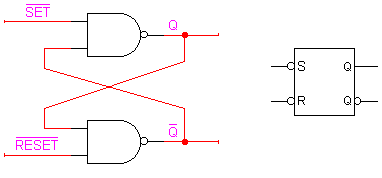
\includegraphics[width=0.5\textwidth]{Exp07/Images/diagram_2.1.png}
  \caption{Latch RS (implementado com \emph{NAND}s)}\label{fig:diagram_2.1.png}
\end{figure}

\textbf{melhorar o texto}\\
A tabela verdade do circuito será a seguinte:

\begin{table}[H]
    \centering
    \caption{Tabela Verdade para \emph{Latch RS}}
    \begin{tabular}{|c|c||c|c|}\hline
      \multicolumn{2}{|c||}{Entradas} & \multicolumn{2}{|c|}{Saídas} \\\hline
      \textbf{A $(\overline{RESET})$} & \textbf{B $(\overline{SET})$} & \textbf{L0 $(Q)$} & \textbf{L1 $(\overline{Q})$} \\\hline
      0 & 0 & 1 & 1 \\\hline
      0 & 1 & 1 & 0 \\\hline
      1 & 0 & 0 & 1 \\\hline
      1 & 1 & $Q_{n}$ & $\overline{Q_{n}}$ \\\hline
    \end{tabular}\label{tab:truth_table_latch_rs}
\end{table}

\href{https://youtu.be/RH6w3QnfUhA}{https://youtu.be/RH6w3QnfUhA}


\textbf{TODO}

% 2.2
\subsection{Latch RS engatilhado}\label{sec:2.2}

\href{https://youtu.be/VNXkBLNcpbo}{https://youtu.be/VNXkBLNcpbo}

Utilizando os modelos de circuitos apresentados temos que sua implementação através do software Deeds será:

\begin{figure}[H]
  \centering
  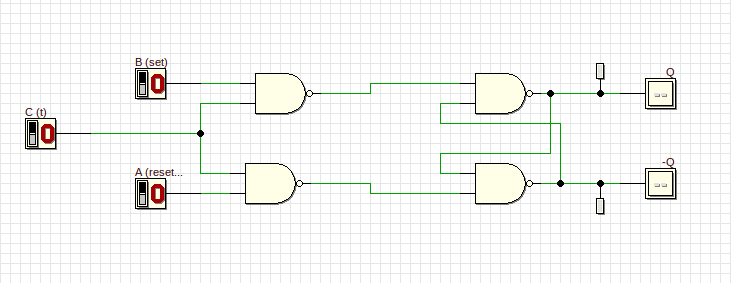
\includegraphics[width=0.8\textwidth]{Exp07/Images/Circ-2.2.png}
  \caption{Latch RS Engatilhado (implementado com \emph{NAND}s)}\label{fig:LatchRS-Engatilhado.png}
\end{figure}

Simulando teremos:
[\href{link-boladão}{\textbf{link-boladão}}]

Sendo que a tabela verdade utilizada será:
\begin{table}[H]
    \centering
    \caption{Tabela Verdade para \emph{Latch RS Engatilhado}}
    \begin{tabular}{|c|c|c||c|c|}\hline
      \multicolumn{3}{|c||}{Entradas} & \multicolumn{2}{|c|}{Saídas} \\\hline
      \textbf{C $({TRIGGER})$} & \textbf{A $({RESET})$} & \textbf{B $({SET})$} & \textbf{L0 $(Q_{n+1})$} & \textbf{L1 $(\overline{Q_{n+1}})$} \\\hline
      0 & X & X & $Q_{n}$ & $\overline{Q_{n}}$ \\\hline
      1 & 0 & 0 & $Q_{n}$ & $\overline{Q_{n}}$\\\hline
      1 & 0 & 1 & 0 & 1\\\hline
      1 & 1 & 0 & 1 & 0 \\\hline
      1 & 1 & 1 & 1 & 1 \\\hline
    \end{tabular}\label{tab:truth_table_latch_rs}
\end{table}

A utilização de um gatilho permite definir quando poderá ocorrer o registro de bits ou não, portanto para $T=0$, temos que o estado das saídas não poderá ser modificado, caso contrário temos a situação em que $T=1$, sendo que este caso descrito possuirá o mesmo comportamento ao utilizar um Latch RS comum.

% 2.3
\subsection{Flip-flop RS}\label{sec:2.3}

\href{link-boladão}{\textbf{link-boladão}}

\textbf{TODO}

% 2.4
\subsection{Flip-flop JK}\label{sec:2.4}

\href{link-boladão}{\textbf{link-boladão}}

\textbf{TODO}

\section{Análise dos Resultados}\label{sec:resultados}

\textbf{TODO}

\subsection{Análise dos tópicos~\ref{sec:2.1} e~\ref{sec:2.2}}\label{sec:analise2.1}

\textbf{TODO}

\subsection{Análise dos tópicos~\ref{sec:2.3}}\label{sec:analise2.4}

\textbf{TODO}

\section{Conclusão}\label{sec:Conclusao}

\textbf{TODO}

\nocite{*}
\bibliographystyle{sbc}
\bibliography{relatorio}  %Aqui é a definição do arquivo .bib a ser usado pelas referências


\newpage
% Colocar aqui apenas as respostas dos itens da Auto-Avaliação
\section*{Auto-Avaliação}

Respostas:

\textbf{TODO}

\begin{table}[H]
      \begin{tabular}{|c|c|} \hline
      \textbf{Questão} & \textbf{Resposta}\\
      \hline
      1  & D \\ \hline
      2  & - \\ \hline
      3  & B \\ \hline
      4  & D \\ \hline
      5  & C \\ \hline
      6  & D \\ \hline
      7  & D \\ \hline
      \end{tabular}
\end{table}


\end{document}
